\section*{Zadanie 9.}
\begin{task}
Fala płaska biegnąca w kierunku $Ox$ i spolaryzowana liniowo tak, że pole elektryczne jest równoległe do osi $Oy$ i ma aplitudę $1\ \cfrac{V}{m}$ pada prostopadle na płytę doskonale przewodzącą, umieszczoną w płaszczyźnie $x=0$. Zapisać rzeczywistą postać wyrażeń na pole $E$ i $H$ dla fali padającej, odbitej i przechodzącej. Obliczyć gęstość powierzchniową prądu płynącego po płycie. Narysować obwiednie pola $E$ i $H$ w otoczeniu płyty. Wyjaśnić, co zmieni się, gdy płyta będzie miała przewodność właściwą $\sigma$ dużą, ale ograniczoną. Narysować obwiednie pól $E$ i $H$ w płycie dla dwóch różnych wartości $\sigma_{1}$ oraz $\sigma{2}=2\sigma_{1}$.\\
\end{task}

\begin{solution}
Postać rzeczywista \textsl{E} i \textsl{H}:
\begin{itemize}
\item $\vec{E^{+}_{1}}=\vec{i_{y}}cos(wt-\beta x)$\\
       $\vec{E^{-}_{1}}=-\vec{i_{y}}cos(wt+\beta x)$\\
       $\vec{E_{2}}=0$
\item $\vec{H^{+}_{1}}=\vec{i_{z}}\cfrac{1}{Z}cos(wt-\beta x)$\\
       $\vec{H^{-}_{1}}=\vec{i_{z}}\cfrac{1}{Z}cos(wt+\beta x)$\\
       $\vec{H_{2}}=0$\\
\end{itemize}
\textbf{Obliczanie gęstości prądu powierzchniowego:}\\
Z warunków brzegowych: $\vec{J_{s}}=\vec{n}\times(\vec{H_{2}}-\vec{H_1})\ \ \implies J_{s}=H_{0}=\cfrac{1}{Z}$

\begin{center}
Obwiednia pól $E$ i $H$ przy padaniu na idealny przewodnik:\\
$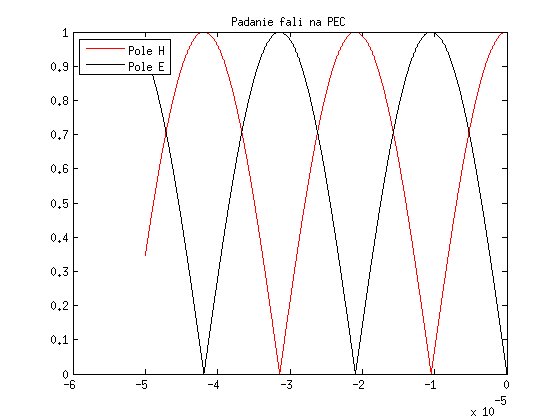
\includegraphics[scale=1]{9_1}$\\

$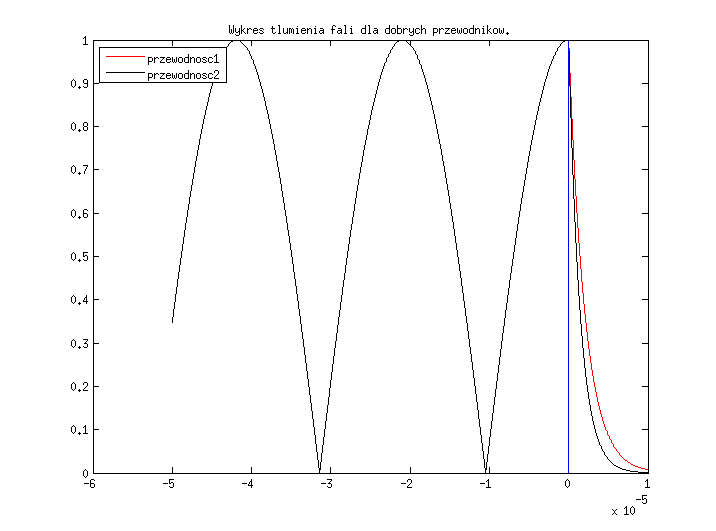
\includegraphics[scale=0.8]{9_2}$\\
\end{center}
Dla dużej ale nie nieskończonej $\sigma$ fale wejdą w przewodnik, ale zostaną bardzo szybko stłumione (skala na osi X na rysunku). Spowoduje to przepływ prądu po bardzo cienkiej powierzchni (ale nie nieskończenie cienkiej) $\rightarrow$ efekt naskórkowy.

\end{solution}